\documentclass[12pt]{article}
\newcommand{\VERSION}{0.0-7}
%\VignetteIndexEntry{gWidgets}
%\VignettePackage{gWidgets}
%\VignetteDepends{methods, gWidgetsRGtk2}

\usepackage{times}              % for fonts
\usepackage[]{geometry}
\usepackage{mathptm}            % for math fonts type 1
\usepackage{graphicx}           % for graphics files
\usepackage{floatflt}           % for ``floating boxes''
%%\usepackage{index}
\usepackage{relsize}            % for relative size fonts
\usepackage{amsmath}            % for amslatex stuff
\usepackage{amsfonts}           % for amsfonts
\usepackage{url}                % for \url,
\usepackage{hyperref}
\usepackage{color}
\usepackage{fancyvrb}
\usepackage{fancyhdr}
\usepackage{jvfloatstyle}       % redefine float.sty for my style. Hack


%% squeeze in stuff
\floatstyle{jvstyle}
\restylefloat{table}
\restylefloat{figure}
\renewcommand\floatpagefraction{.9}
\renewcommand\topfraction{.9}
\renewcommand\bottomfraction{.9}
\renewcommand\textfraction{.1}
\setcounter{totalnumber}{50}
\setcounter{topnumber}{50}
\setcounter{bottomnumber}{50}

%% Fill these in
\pagestyle{fancy}
\usepackage{fancyhdr}
\pagestyle{fancy}
\fancyhf{}
\fancyhead[L]{\RCode{gWidgets}}
\fancyhead[C]{}
\fancyhead[R]{\sectionmark}
\fancyfoot[L]{}
\fancyfoot[C]{- page \thepage\/ -}
\fancyfoot[R]{}
\renewcommand{\headrulewidth}{0.1pt}
\renewcommand{\footrulewidth}{0.0pt}

%% My abbreviations
\newcommand{\RCode}[1]{\texttt{#1}}
\newcommand{\RFunc}[1]{\texttt{#1()}}
\newcommand{\RPackage}[1]{\textbf{#1}}
\newcommand{\RArg}[1]{\texttt{#1=}}
\newcommand{\RListel}[1]{\texttt{\$#1}}


\newenvironment{RArgs}{\begin{list}{}{}}{\end{list}}


\usepackage{/usr/local/R/lib/R/share/texmf/Sweave}
\begin{document}
\thispagestyle{plain}
\title{Examples for gWidgets}

\author{John Verzani, \url{gWidgetsRGtk@gmail.com}}
\maketitle

\section*{Abstract:}
Examples for using the \RPackage{gWidgets} package are presented. Th
\RCode{gWidgets} API is intended to be a cross platform means to
interact with a graphics toolkit. Currently, the only available
toolkit is the GTK toolkit via the \RPackage{gWidgetsRGtk2} package
which uses the \RPackage{RGtk2} package. Although not nearly as
powerful as any individual toolkit, the \RPackage{gWidgets} API is
suitable for many tasks or as a rapid prototyping tool for more
complicated applications. Hopefully the examples contained herein
illustrate that quite a few things can be done fairly easily, and
complicated things pieced together in a straightforward manner. To see
an application built using \RPackage{gWidgets}, install the
\RPackage{pmg} GUI (\url{http://www.math.csi,cuny.edu/pmg}).

\setcounter{tocdepth}{3}
\tableofcontents

\section{Background}
The \RPackage{gWidgetsRGtk2} package implements the \RCode{gWidgets} API for the
GTK toolkit. The GTK toolkit is interfaced using the \RPackage{RGtk2}
package of Michael Lawrence, in turn derived from Duncan Temple Lang's
\RPackage{RGtk} package. The excellent \RPackage{RGtk2} package opens up
the full power of the GTK2 toolkit, only a fraction of which is
available though \RPackage{gWidgetsRGtk2}.  The \RCode{gWidgets} API is intended
to be a cross-toolkit API for working with GUI objects. It is based on
the iwidgets API of Simon Urbanek, with improvement by Philippe
Grosjean, Michael Lawrence, Simon Urbanek and John Verzani.

The \RCode{gWidgets} API is still in the formative stages and likely will
change as more people use it and offer suggestions for improvement.

We  load the \RCode{gWidgets} package, using the \RCode{gWidgetsRGtk2}
toolkit, below. When \RCode{gWidgets} is started, it will ask you to choose
between toolkit implementations, if more than one is available. If the
option \RCode{guiToolkit} is set to a package name, less the
``gWidgets'' then that package will be used. 
following 
\begin{Schunk}
\begin{Sinput}
> options(guiToolkit = "RGtk2")
> require(gWidgets)
\end{Sinput}
\begin{Soutput}
[1] TRUE
\end{Soutput}
\end{Schunk}


Both the \RPackage{gWidgets} and \RPackage{gWidgetsRGtk2} package use
S4 methods and classes and load much faster under the newer
\RPackage{methods} package accompanying R version 2.4.0 or greater.

This document supplements the man pages by providing more detailed
examples. The man pages contain more specific information. See the 
page \RCode{gWidgets-package} for a listing of the available man pages.

This document is a vignette. As such, the code displayed is available
within an R session through the command
\RCode{edit(vignette("gWidgets"))}. 


\section{Installation}
In case you are reading this vignette without having installed
gWidgets, here are some instructions. As only the
\RCode{gWidgetsRGtk2} package is available to interface with a
toolkit, I'll describe how this is installed.

Installing \RCode{gWidgets} with the \RCode{gWidgetsRGtk2} pakcage
requires two steps: installing the GTK libraries and installing the R
packages.



\subsection{Installing the GTK libraries}

The \RCode{gWidgetsRGtk2} provides a link between \RCode{gWidgets} and
the GTK libraries through the \RCode{RGTk2} package.  \texttt{RGtk2}
requires relatively modern versions of the GTK libraries (2.8.0 or
higher). These may need to be installed or upgraded on your system.

In case of \textbf{Windows} do this:

\begin{enumerate}
\item 
 Download the files from
\href{http://gladewin32.sourceforge.net/modules/wfdownloads/visit.php?lid=102}{http://gladewin32.sourceforge.net/modules/wfdownloads/visit.php?lid=102}

\item run the resulting file.  This is an automated installer which will walk
you through the installation of the Gtk2 libraries.
\end{enumerate}

In Linux, you may or may not need to upgrade the GTK libraries
depending on your distribution.

For Mac OS X, I've installed the GTK libraries from source on my older
10.3.9 machine using Apples X11 server. You may be able to use FINK
now, but this is not tested.


For more details on RGtk2 refer to
\href{http://www.ggobi.org/rgtk2}{RGtk2's home page}.


\subsection{Install the R packages}

The following R packages are needed: \texttt{RGtk2},
\texttt{cairoDevice}, \texttt{gWidgets}, and \texttt{gWidgetsRGtk2}
\texttt{pmg}. Install them in this order, as some depend on others to
be installed first. All can be downloaded from CRAN.

These can all be installed by following the dependencies for
\RCode{gWidgetsRGtk2}. The following command may work for you:

\begin{verbatim}
   install.packages("gWidgetsRGtk2", dep = TRUE)
\end{verbatim}

You may need to adjust the location where the libraries will be
installed if you do not have the proper permissions.

For MAC OS X, the packages are source, not the default ``mac.binary.'' Try
\begin{verbatim}
   install.packages("gWidgetsRGtk2", dep = TRUE,type = "source" )
\end{verbatim}

The newest versions will be on
\href{http://www.math.csi.cuny.edu/pmg}{gWidgets's website}. To install
from here add the \texttt{repos=} argument, as follows:

\begin{verbatim}
> install.packages("gWidgetsRGtk2",dep = TRUE, repos = "http://www.math.csi.cuny.edu/pmg")
\end{verbatim}



\section{Hello world}

We begin by showing how to make various widgets which display the
ubiquitous ``Hello world'' message. First though we define a function
allowing us to comment code within Sweave.
\begin{Schunk}
\begin{Sinput}
> Comment = function(...) invisible(...)
\end{Sinput}
\end{Schunk}




\begin{figure}[htbp]
  \centering
  \begin{tabular}{l@{\quad}l}
  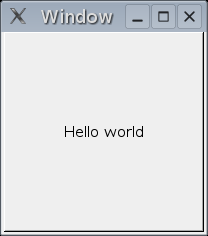
\includegraphics[width=.35\textwidth]{button}&
  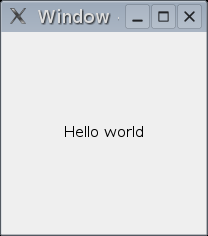
\includegraphics[width=.35\textwidth]{label}\\
  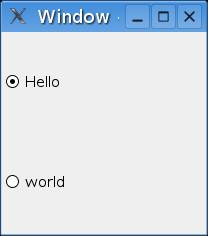
\includegraphics[width=.35\textwidth]{radio}&
  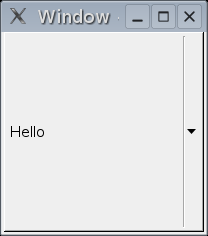
\includegraphics[width=.35\textwidth]{droplist}
  \end{tabular}
  \caption{Four basic widgets: a button, a label, radio buttons, and a drop list.}
  \label{fig:basic-widgets}
\end{figure}


Now to illustrate (Figure~\ref{fig:basic-widgets} shows a few) some of
the basic widgets.
These first widgets display text: a label, a button and a text area.


First a button:
\begin{Schunk}
\begin{Sinput}
> obj = gbutton("Hello world", container = gwindow())
\end{Sinput}
\end{Schunk}

Next a label:
\begin{Schunk}
\begin{Sinput}
> obj = glabel("Hello world", container = gwindow())
\end{Sinput}
\end{Schunk}

Now for single line of ediable text:
\begin{Schunk}
\begin{Sinput}
> obj = gedit("Hello world", container = gwindow())
\end{Sinput}
\end{Schunk}

Finally, a text buffer for multiple lines of text:
\begin{Schunk}
\begin{Sinput}
> obj = gtext("Hello world", container = gwindow())
\end{Sinput}
\end{Schunk}

The following widgets are used for selection of a value or values from
a vector of possible values.

First a radio group for selecting just one:
\begin{Schunk}
\begin{Sinput}
> obj = gradio(c("hello", "world"), container = gwindow())
\end{Sinput}
\end{Schunk}

Next, a drop list, or combo box, again for selecting just one,
although in this case an optin can be give for the user to edit the value.
\begin{Schunk}
\begin{Sinput}
> obj = gdroplist(c("hello", "world"), container = gwindow())
\end{Sinput}
\end{Schunk}

For longer lists, a table of values can be used.
\begin{Schunk}
\begin{Sinput}
> obj = gtable(c("hello", "world"), container = gwindow())
\end{Sinput}
\end{Schunk}
This widget is also used for displaying tabular data with multiple
columns and rows.  This widget an argument allowing for multiple
selections. Such selection can also be achieved with a checkbox group:

\begin{Schunk}
\begin{Sinput}
> obj = gcheckboxgroup(c("hello", "world"), container = gwindow())
\end{Sinput}
\end{Schunk}



For selecting a numeric value, sliders and spinbuttons are commonly used:
\begin{Schunk}
\begin{Sinput}
> obj = gslider(from = 0, to = 7734, by = 100, value = 0, container = gwindow())
> obj = gspinbutton(from = 0, to = 7734, by = 100, value = 0, container = gwindow())
\end{Sinput}
\end{Schunk}
Both these widgets are used to select a value from a prespecified
sequence of numbers.


Common to all of the above is a specification of the ``value'' of the
widget, and the container to attach the widget to. In each case a
top-level window constructed by \RFunc{gwindow}.


In this next example, we show how to  combine widgets together using
containers. (Figure~\ref{fig:hello-world}.)


\begin{Schunk}
\begin{Sinput}
> win = gwindow("Hello World, ad nauseum", visible = TRUE)
> group = ggroup(horizontal = FALSE, container = win)
> obj = gbutton("Hello...", container = group, handler = function(h, 
+     ...) gmessage("world"))
> obj = glabel("Hello...", container = group, handler = function(h, 
+     ...) gmessage("world"))
> obj = gdroplist(c("Hello", "world"), container = group)
> obj = gedit("Hello world", container = group)
> obj = gtext("Hello world", container = group, font.attr = list(style = "bold"))
\end{Sinput}
\end{Schunk}


As before, the constructors \RFunc{gbutton}, \RFunc{glabel},
\RFunc{gedit} and \RFunc{gtext} create widgets of different types.
The button looks like a button. A label is used to show text which may
perhaps be edited. A droplist allows a user to select one of several
items, or if desired to be able to add a value. The \RFunc{gedit} and
\RFunc{gtext} constructors both create widgets for inputting text, in
the first case for single lines, and in the second for multiple lines
using a text buffer.

\begin{figure}[htbp]
  \centering
  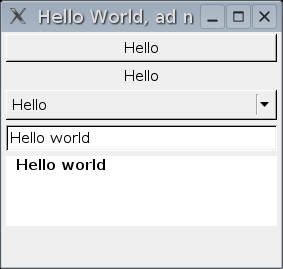
\includegraphics[width=.35\textwidth]{helloWorld}
  \caption{Hello world example}
  \label{fig:hello-world}
\end{figure}

These widgets are packed into containers (see \RCode{?ggroup} or
\RCode{?gwindow}). The base container is a window, created with the
\RFunc{gwindow} function. A window can only contain one widget, so
we pack in a group container created with \RFunc{ggroup}. The
\RFunc{ggroup} container packs in widgets from left to right or top to
bottom. Imagine each widget as a block which is added to the
container.  In this case, we want the subsequent widgets packed in top
to bottom so we used the argument \RCode{horizontal=FALSE}.

For the button and label widgets, a  handler is set so that when the widget is
clicked a message dialog appears showing ``world.'' Handlers are used
to respond to mouse-driven events. In this case the event of a widget
being clicked. See \RCode{?gWidgetsRGtk-handlers} for details on
handlers. 

The message is an instance of a dialog. in the \RPackage{gWidgets} API
dialogs are usually modal, meaning nothing can be done until they are
dismissed. (This can be annoying if a dialog appears under another
window and can't be seen!)


\section{Making a confirmation dialog}

Let's see how we might use widgets to create our own confirmation
dialog. We want to have an icon, a label for the message, and  buttons
to confirm or dismiss the dialog.

The \RFunc{gimage} constructor allows images to be shown in a
widget. In \RPackage{gWidgetsRGtk} there are several stock images, which can be
listed with \RFunc{getStockIcons}. We will use ``info'' below.

First we define a function for making a dialog. This one uses
nested group containers to organize the layout. Alternately the
\RFunc{glayout} constructor could have been used in some manner.

\begin{Schunk}
\begin{Sinput}
> confirmDialog = function(message, handler = NULL) {
+     window = gwindow("Confirm")
+     group = ggroup(container = window)
+     add(group, gimage("info", dirname = "stock", size = "dialog"))
+     Comment("A group for the message and buttons")
+     innner.group = ggroup(horizontal = FALSE, container = group)
+     add(innner.group, glabel(message), expand = TRUE)
+     Comment("A group to organize the buttons")
+     button.group = ggroup(container = innner.group)
+     Comment("Push buttons to right")
+     addSpring(button.group)
+     obj = gbutton("ok", handler = handler, container = button.group)
+     obj = gbutton("cancel", handler = function(h, ...) dispose(window), 
+         container = button.group)
+     return()
+ }
\end{Sinput}
\end{Schunk}

The key to making a useful confirmation dialog is attaching an action
to the ``ok'' button. This is done with the argument
\RArg{handler}. Below, this function prints a message and then
closes the dialog. To do this, the \RFunc{dispose} method is called on
the ``ok'' button  widget, which is referenced inside the handler by
\RCode{h\$obj} below. In \RCode{gWidgets}, handlers are passed
information via the first argument, which is a list with named
elements. The \RListel{obj} component refers to the widget the handler
is assigned to. 

Trying it out produces a widget like that shown in Figure~\ref{fig:confirmDialog}

\begin{figure}[htbp]
  \centering
  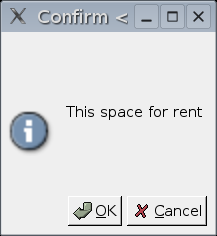
\includegraphics[width=.35\textwidth]{confirmDialog}
  \caption{Confirmation dialog}
  \label{fig:confirmDialog}
\end{figure}

\begin{Schunk}
\begin{Sinput}
> confirmDialog("This space for rent", handler = function(h, ...) {
+     print("what to do... [Change accordingly]")
+     Comment("In this instance dispose finds its parent window and closes it")
+     dispose(h$obj)
+ })
\end{Sinput}
\begin{Soutput}
NULL
\end{Soutput}
\end{Schunk}
%%$

\section{Methods}

Widgets are interacted with by their methods. The main methods are
\RFunc{svalue} and \RFunc{svalue<-} for getting and setting a widgets
primary value. 

The following silly example illustrates how clicking one widget can be
used to update another widget.
\begin{Schunk}
\begin{Sinput}
> group = ggroup(container = gwindow("Two widgets"))
> widget1 = gbutton("Click me to update the counter", container = group, 
+     handler = function(h, ...) {
+         oldVal = svalue(widget2)
+         svalue(widget2) <- as.numeric(oldVal) + 1
+     })
> widget2 = glabel(0, container = group)
\end{Sinput}
\end{Schunk}
The value stored in a label is just the text of the label. This is
returned by \RFunc{svalue} and after 1 is added to the value, replaced
back into the label. As text labels are of class ``character,'' the
value is coerced to be numeric.

There are other methods (see \RCode{?gWidgetsRGtk-methods}) that try
to make interacting with a widget as natural as possible. For
instance, a radio button has a selected value returned by
\RFunc{svalue}, but also a vector of possible values. These may be
referenced using vector, \RCode{[}, notation.

\section{Adding a GUI to some common  tasks}

A GUI can make some command line tasks easier to perform. Here are a
few examples that don't involve much coding in \RCode{gWidgets}.

\subsection{\RFunc{file.choose}}
The \RFunc{file.choose} function is great for simplifying a user's
choice of a file from the file system. A typical usage might be
\begin{Soutput}
  source(file.choose())
\end{Soutput}
to allow a user to source a file with a little help from a
GUI. However, in many UNIX environments, there is no GUI for
\RFunc{file.choose}, only a more convenient curses interface. With the
\RFunc{gfile} dialog, we can offer some improvement.

We have to reverse our thinking though. The command
\RCode{source(file.choose())} acts like function composition -- the
output of \RFunc{file.choose} is sent to \RFunc{source}. We
instead give a handler to \RFunc{gfile} to process the selected
file. Below is a function written to give some flexibility to the
process.

\begin{Schunk}
\begin{Sinput}
> fileChoose = function(action = "print", text = "Select a file...", 
+     type = "open", ...) {
+     gfile(text = text, type = type, ..., action = action, handler = function(h, 
+         ...) {
+         do.call(h$action, list(svalue(h$obj)))
+     })
+ }
\end{Sinput}
\end{Schunk}

Now various tasks can be done quite simply. To \RFunc{source} a file
we have
\begin{Sinput}
> fileChoose(action="source")
\end{Sinput}

Or to set the   current working directory we have
\begin{Sinput}
>  fileChoose(action="setwd", type="selectdir", text="Select a directory...")
\end{Sinput}

\subsection{\RFunc{browseEnv}}
\label{sec:browseEnv}

The \RFunc{browseEnv} function craetes a table in a web browser
listing the current objects in the global environement (by default)
and details some properties of them. This is an easy to use function,
but suffers from the fact that it may have to open up a browser for
the user if none is already open. This may take a bit of time as
browsers are generally slow to load. We illustrate a means of using
the \RFunc{gtable} constructor to show in a table the objects in an
environment.

The following function creates the data.frame we will display. Consult the code
of \RFunc{browseEnv} to see how to produce more details.

\begin{Schunk}
\begin{Sinput}
> lstObjects = function(envir = .GlobalEnv, pattern) {
+     objlist = ls(envir = envir, pattern = pattern)
+     objclass = sapply(objlist, function(objName) {
+         obj <- get(objName, envir = envir)
+         class(obj)[1]
+     })
+     data.frame(Name = I(objlist), Class = I(objclass))
+ }
\end{Sinput}
\end{Schunk}

Now to make a table to display the results. We leave some flexibility
with the arguments, although we won't illustrate this.


\begin{Schunk}
\begin{Sinput}
> browseEnv1 = function(envir = .GlobalEnv, pattern) {
+     listOfObjects = lstObjects(envir = envir, pattern)
+     gtable(listOfObjects, container = gwindow("browseEnv1"), 
+         )
+ }
\end{Sinput}
\end{Schunk}

Tables can have a double click handler (a single click is used for
selection). To illustrate, we  add a handler which 
calls \RFunc{summary} (or some other function) on a double-clicked item.

\begin{Schunk}
\begin{Sinput}
> browseEnv2 = function(envir = .GlobalEnv, pattern, action = "summary") {
+     listOfObjects = lstObjects(envir = envir, pattern)
+     gtable(listOfObjects, container = gwindow("browseEnv2"), 
+         action = action, handler = function(h, ...) {
+             print(do.call(h$action, list(svalue(h$obj))))
+         })
+ }
\end{Sinput}
\end{Schunk}

As a final refinement, we  add a droplist box to filter by the unique
values of ``Class.'' We leave as an excercise the display of icons
based on the class of the object.
\begin{Schunk}
\begin{Sinput}
> browseEnv3 = function(envir = .GlobalEnv, pattern, action = "summary") {
+     listOfObjects = lstObjects(envir = envir, pattern)
+     gtable(listOfObjects, container = gwindow("browseEnv3"), 
+         filter.column = 2, action = action, handler = function(h, 
+             ...) {
+             print(do.call(h$action, list(svalue(h$obj))))
+         })
+ }
\end{Sinput}
\end{Schunk}

The \RFunc{gvarbrowser} function constructs a widget very similar to
this, only it uses \RFunc{gtree} to allow further display of
list-like objects.


\section{A gWidgetsDensity demo}
\label{sec:repeating-plot}

We illustrate how to make a widget to dynamically update a density
plot. The idea comes from the \RCode{tkdensity} demo that accompanies
the \RPackage{tcltk} package.

We use the  \RFunc{ggraphics} constructor to create a new plot device. For
RGtk2, this uses the \RPackage{cairoDevice} package also developed
by Michael Lawrence.

The demo consists of a widget to control a random sample, in this case
from the standard normal distribution or the exponential distribution
with rate 1; a widget to select the sample size; a widget to select the
kernel; and a widget to adjust the default bandwidth. We use radio
buttons for the first two, a drop list for the third and a slider for
the latter.

Proceeding, first we define the two distributions and the possible kernels.
\begin{Schunk}
\begin{Sinput}
> availDists = c(Normal = "rnorm", Exponential = "rexp")
> availKernels = c("gaussian", "epanechnikov", "rectangular", "triangular", 
+     "biweight", "cosine", "optcosine")
\end{Sinput}
\end{Schunk}

We then define the key function for drawing the graphic. This refers
to widgets yet to be defined.
                      
\begin{Schunk}
\begin{Sinput}
> updatePlot = function(h, ...) {
+     x = do.call(availDists[svalue(distribution)], list(svalue(sampleSize)))
+     plot(density(x, adjust = svalue(bandwidthAdjust), kernel = svalue(kernel)), 
+         main = "Density plot")
+     rug(x)
+ }
\end{Sinput}
\end{Schunk}
Now to define the widgets.
\begin{Schunk}
\begin{Sinput}
> distribution = gradio(names(availDists), horizontal = FALSE, 
+     handler = updatePlot)
> kernel = gdroplist(availKernels, handler = updatePlot)
> bandwidthAdjust = gslider(from = 0, to = 2, by = 0.01, value = 1, 
+     handler = updatePlot)
> sampleSize = gradio(c(50, 100, 200, 300), handler = updatePlot)
\end{Sinput}
\end{Schunk}

And now the layout. We use frames to set off the different
arguments. A frame is like a group, only it has an option for placing
a text label somewhere along the top, with a default using the left-hand
side.
\begin{Schunk}
\begin{Sinput}
> window = gwindow("gWidgetsDensity")
> BigGroup = ggroup(cont = window)
> group = ggroup(horizontal = FALSE, container = BigGroup)
> tmp = gframe("Distribution", container = group)
> add(tmp, distribution)
> tmp = gframe("Sample  size", container = group)
> add(tmp, sampleSize)
> tmp = gframe("Kernel", container = group)
> add(tmp, kernel)
> tmp = gframe("Bandwidth adjust", container = group)
> add(tmp, bandwidthAdjust, expand = TRUE)
\end{Sinput}
\end{Schunk}

Now to add a graphics device.
\begin{Soutput}
> add(BigGroup, ggraphics())
\end{Soutput}


A realization of this widget was captured in Figure~\ref{fig:gtkdensity}.

\begin{figure}
  \centering
  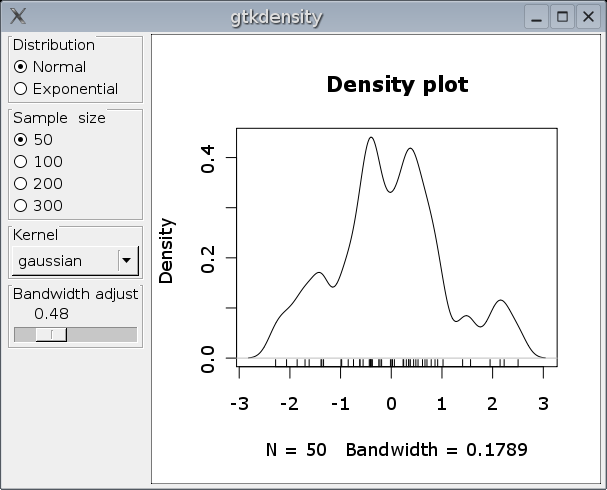
\includegraphics[width=.6\textwidth]{gtkdensity}
  \caption{The gWidgetsDensity example in action.}
  \label{fig:gtkdensity}
\end{figure}



\section{Composing email}

We next give an example of how to write a widget for composing an
email message. Not that this is what R is intended for, but rather to
show how a familiar widget is produced by combining various pieces
from \RCode{gWidgets}. This example is a little lengthy (especially
with Sweave's formatting), but hopefully straightforward due to the
familiarity with the result of the task.

For our stripped-down compose window we want the following: a menubar
to organize functions; a toolbar for a few common functions; a ``To:''
field which should have some means to store previously used e-mails; a
``From:'' field that should be editable, but not obviously so as often
it isn't edited; a ``Subject:'' field which also updates the title of
the window; and a text buffer for typing the message.

The following code will create a function called \RFunc{Rmail}
(apologies to old-time emacs users) which on many UNIX machines can
send out e-mails using the \RCode{sendmail} command.

First we define some variables:
\begin{Schunk}
\begin{Sinput}
> FROM = "gWidgetsRGtk <gWidgetsRGtk@gmail.com>"
> buddyList = c("My Friend <myfriend@gmail.com>", "My dog <mydog@gmail.com>")
\end{Sinput}
\end{Schunk}

Now for the main function. We define some helper functions inside the
body, so as not to worry about scoping issues.
\begin{Schunk}
\begin{Sinput}
> Rmail = function(draft = NULL, ...) {
+     Comment("Define main widgets, store in a list for ease of use")
+     widgets = list()
+     widgets$to = gdroplist(c(), editable = TRUE)
+     widgets$from = glabel(FROM, editable = TRUE)
+     widgets$subject = gedit()
+     widgets$text = gtext()
+     Comment("Handle drafts. Either a list or a filename to source")
+     Comment("The generic svalue() method makes setting values easy")
+     if (!is.null(draft)) {
+         if (is.character(draft)) 
+             source(draft)
+         if (is.list(draft)) 
+             sapply(c("to", "from", "subject", "text"), function(i) svalue(widgets[[i]]) <- draft[[i]])
+     }
+     Comment("Helper functions")
+     sendIt = function(...) {
+         tmp = tempfile()
+         cat("To:", svalue(widgets$to), "\n", file = tmp, append = TRUE)
+         cat("From:", svalue(widgets$from), "\n", file = tmp, 
+             append = TRUE)
+         cat("Subject:", svalue(widgets$subject), "\n", file = tmp, 
+             append = TRUE)
+         cat("Date:", format(Sys.time(), "%d %b %Y %T %Z"), "\n", 
+             file = tmp, append = TRUE)
+         cat("X-sender:", "R", file = tmp, append = TRUE)
+         cat("\n\n", file = tmp, append = TRUE)
+         cat(svalue(widgets$text), file = tmp, append = TRUE)
+         cat("\n", file = tmp, append = TRUE)
+         Comment("Use UNIX sendmail to send message")
+         system(paste("sendmail -t  <", tmp))
+         Comment("Add To: to buddyList")
+         if (exists("buddyList")) 
+             assign("buddyList", unique(c(buddyList, svalue(widgets$to))), 
+                 inherits = TRUE)
+         Comment("Close window, delete file")
+         unlink(tmp)
+         dispose(window)
+     }
+     Comment("Function to save a draft to the file draft.R")
+     saveDraft = function(...) {
+         draft = list()
+         sapply(c("to", "from", "subject", "text"), function(i) draft[[i]]) <- svalue(widgets[[i]])
+         dump("draft", "draft.R")
+         cat("Draft dumped to draft.R\n")
+     }
+     Comment("A simple dialog")
+     aboutMail = function(...) gmessage("Sends a message")
+     Comment("Make main window from top down")
+     window = gwindow("Compose mail")
+     group = ggroup(horizontal = FALSE, spacing = 0, container = window)
+     Comment("Remove border")
+     svalue(group) <- 0
+     Comment("Menubar is defined by a list")
+     menubarlist = list()
+     menubarlist$File$Save$handler = saveDraft
+     menubarlist$File$Send$handler = sendIt
+     menubarlist$File$Quit$handler = function(...) dispose(window)
+     menubarlist$File$Quit$icon = "quit"
+     menubarlist$Help$About$handler = aboutMail
+     add(group, gmenu(menubarlist))
+     Comment("Toolbar is also defined by a list")
+     toolbarlist = list()
+     toolbarlist$Send$handler = sendIt
+     toolbarlist$Send$icon = "connect"
+     toolbarlist$Save$handler = saveDraft
+     toolbarlist$Save$icon = "save"
+     add(group, gtoolbar(toolbarlist))
+     Comment("Put headers in a glayout() container")
+     tbl = glayout(container = group)
+     Comment("To: field. Looks for buddyList")
+     tbl[1, 1] = glabel("To:")
+     tbl[1, 2] = widgets$to
+     if (exists("buddyList")) 
+         widgets$to[] <- buddyList
+     Comment("From: field. Click to edit value")
+     tbl[2, 1] = glabel("From:")
+     tbl[2, 2] = widgets$from
+     Comment("Subject: field. Handler updates window title")
+     tbl[3, 1] = glabel("Subject:")
+     tbl[3, 2] = widgets$subject
+     addhandlerkeystroke(widgets$subject, handler = function(h, 
+         ...) svalue(window) = paste("Compose mail:", svalue(h$obj), 
+         collapse = ""))
+     Comment("Layout needs to be finalized")
+     visible(tbl) <- TRUE
+     Comment("Add text box for message, but first some space")
+     addSpace(group, 5)
+     add(group, widgets$text, expand = TRUE)
+     Comment("That's it.")
+ }
\end{Sinput}
\end{Schunk}
%%$

To compose an e-mail we call the function as follows. (The widget constructed looks like Figure~\ref{fig:Rmail}.)
\begin{Schunk}
\begin{Sinput}
> Rmail()
\end{Sinput}
\end{Schunk}

\begin{figure}[htbp]
  \centering
  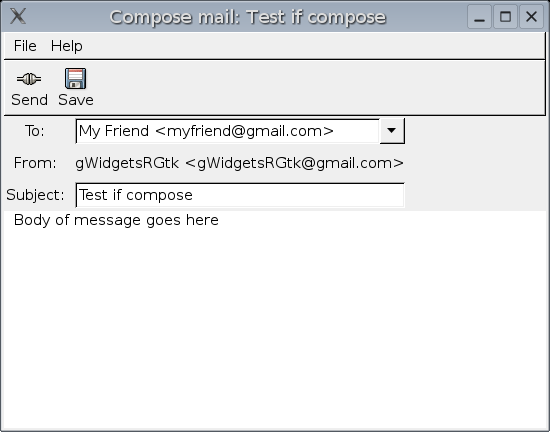
\includegraphics[width=.5\textwidth]{Rmail}
  \caption{Widget for composing an e-mail message }
  \label{fig:Rmail}
\end{figure}

The \RFunc{Rmail} function uses a few  tricks.  A droplist is
used to hold the ``To:'' field. This is done so that a ``buddy list''
can be added if present. The \RCode{[<-} method for drop lists make
this straightforward. For widgets that have a collection of items to
select from, the vector and matrix methods are defined to make
changing values familiar to R users.

The ``From:'' field uses an editable label. Clicking in the label's
text allows its value to be changed. Just hit ENTER when done.

The handler assigned to the ``Subject:'' field updates the window
title every keystroke. The title of the window is updated with the windows
\RFunc{svalue<-} method.

The \RFunc{svalue} and \RFunc{svalue<-} methods are the work-horse
methods of \RCode{gWidgets}. The are used to retrieve the selected
value of a widget or set the selected value of a widget. One advantage
to have a single generic function do this is illustrated in the
handling of a draft:
\begin{Soutput}
 sapply(c("to","from","subject","text"), function(i)
   svalue(widgets[[i]]) <- draft[[i]])
\end{Soutput}

As for the \RFunc{sendIt} function, this is just one way to send an
e-mail message on a UNIX machine. There are likely more than 100
different ways people could think of doing this task, most better than
this one.

\section{Drag and drop}
GTK supports drag and drop features, and \RCode{gWidgets} provides a
simple mechanism to add drag and drop to widgets. (Some widgets, such
as text boxes, support drag and drop without these.) The basic
approach is to add a drop source to the widget you wish to drag from,
and add a drop target to the widget you want to drag to. You can also
provide a handler to deal with motions over the drop target. See the
man page \RCode{?gWidgetsRGtk-dnd} for more information.

We give two examples of drag and drop. One where variables from the
variable browser are dropped onto a graph widget. Another illustrating
drag and drop from the data frame editor to a widget.

\subsection{DND with plots}


This example shows the use of the plot device, the variable browser
widget, and the use of the drag and
drop features of gWidgets (Figure~\ref{fig:doPlot}).



\begin{Schunk}
\begin{Sinput}
> doPlot = function() {
+     Comment("Set up main group")
+     mainGroup = ggroup(container = gwindow("doPlot example"))
+     Comment("The variable browser widget")
+     gvarbrowser(container = mainGroup)
+     rightGroup = ggroup(horizontal = FALSE, container = mainGroup)
+     Comment("The graphics device")
+     ggraphics(container = rightGroup)
+     entry = gedit("drop item here to be plotted", container = rightGroup)
+     adddroptarget(entry, handler = function(h, ...) {
+         do.call("plot", list(svalue(h$dropdata), main = id(h$dropdata)))
+     })
+ }
\end{Sinput}
\end{Schunk}
%%$
\begin{Soutput}
> doPlot()
\end{Soutput}


\begin{figure}[htbp]
  \centering
  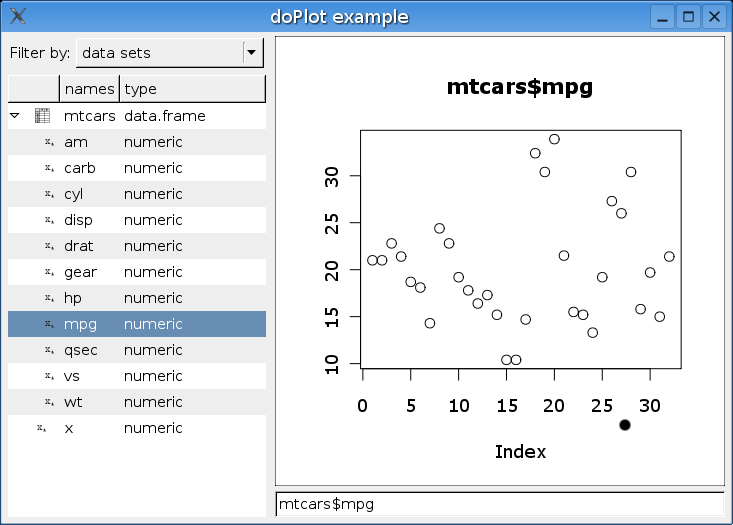
\includegraphics[width=.6\textwidth]{doPlot}
  \caption{Dialog produced by \RFunc{doPlot} example}
  \label{fig:doPlot}
\end{figure}

The basic structure of using \RCode{gWidgets} is present in this
example. The key widgets are the variable browser
(\RFunc{gvarbrowser}), the plot device (\RFunc{ggraphics}), and the
text-entry widget (\RFunc{gedit}). These are put into differing
containers.  Finally, there is an handler given to the result of the
drag and drop. The \RFunc{do.call} line uses the \RFunc{svalue} and
\RFunc{id} methods on a character, which in this instance return the
variable with that name and the name.


To use this widget, one drags a variable to be plotted from the
variable browser over to the area below the plot window. The
\RFunc{plot} method is called on the values in the dropped variable.


\subsection{DND from the data frame editor}
The \RFunc{gdf} constructor makes a widget for editing data
frames. The columns of which can be dropped onto a widget. This is
done by dragging the column header. The code below also adds a handler
so that changes to the column propogate to changes in the widget where
the column is dropped. This has some issues, as the handler needs to
be removed if the widget is closed.

\begin{Schunk}
\begin{Sinput}
> Comment("Drag a column onto plot to have a boxplot drawn.")
> Comment("Changing the column values will redraw the graph.")
> makeDynamicWidget = function() {
+     win = gwindow("Draw a boxplot")
+     gd = ggraphics(container = win)
+     adddroptarget(gd, targetType = "object", handler = function(h, 
+         ...) {
+         tag(gd, "data") <- h$dropdata
+         plotWidget(gd)
+         Comment("this makes the dynamic part:")
+         Comment("- we put a change handler of the column that we get the data from")
+         Comment("- we store the handler id, so that we can clean up the handler when this")
+         Comment("  window is closed")
+         Comment("The is.gdataframecolumn function checks if the drop value")
+         Comment("  comes from the data frame editor (gdf)")
+         if (is.gdataframecolumn(h$dropdata)) {
+             view.col = h$dropdata
+             Comment("Put change handler on column to update plotting widget")
+             id = addhandlerchanged(view.col, handler = function(h, 
+                 ...) plotWidget(gd))
+             Comment("Save drop handler id so that it can be removed when")
+             Comment("  widget  is closed")
+             dropHandlers = tag(gd, "dropHandlers")
+             dropHandlers[[length(dropHandlers) + 1]] = list(view.col = view.col, 
+                 id = id)
+             tag(gd, "dropHandlers") <- dropHandlers
+         }
+     })
+     Comment("Remove drop handlers if widget is unrealized.")
+     addhandlerunrealize(gd, handler = function(h, ...) {
+         dropHandlers = tag(gd, "dropHandlers")
+         if (length(dropHandlers) > 0) {
+             for (i in 1:length(dropHandlers)) {
+                 removehandler(dropHandlers[[i]]$view.col, dropHandlers[[i]]$id)
+             }
+         }
+     })
+ }
\end{Sinput}
\end{Schunk}

Next, we make the function that produces or updates the graphic. The
data is stored in the tag-key "data". The use of \RFunc{id} and
\RFunc{svalue} works for values which are either variable names or columns.

\begin{Schunk}
\begin{Sinput}
> plotWidget = function(widget) {
+     data = tag(widget, "data")
+     theName = id(data)
+     values = svalue(data)
+     boxplot(values, xlab = theName, horizontal = TRUE, col = gray(0.75))
+ }
\end{Sinput}
\end{Schunk}

Now show the two widgets, the \RFunc{gdf} function constructs the data
frame editor widget.
\begin{Soutput}
> gdf(mtcars, container=TRUE)
> makeDynamicWidget()
\end{Soutput}
%%$


\section{Notebooks}

The notebook is a common metaphor with computer applications, as they
can give access to lots of information compactly on the screen. The
\RFunc{gnotebook} constructor produces a notebook
widget. New pages are added via the \RFunc{add} method, the current
page is deleted through an icon, or via the \RFunc{dispose} method,
and vector methods are defined, such as \RFunc{names}, to make
interacting with notebooks natural.

The following example shows how a notebook can be used to organize
different graphics devices. (See the \RFunc{ggraphicsnotebook} function
for a similar widget.)

Our widget consists of a toolbar to add or delete plots and a notebook
to hold the different graphics devices. The basic widgets are defined
by the following:

First we make window and group containers to hold our widgets and then
a notebook instance.
\begin{Schunk}
\begin{Sinput}
> win = gwindow("Plot notebook")
> group = ggroup(horizontal = FALSE, container = win)
> nb = gnotebook()
\end{Sinput}
\end{Schunk}
Next, we begin with an initial plot device.
\begin{Soutput}
> add(nb, ggraphics(), label="plot")
\end{Soutput}
The \RFunc{add} method is used to add new widgets, in this case a
graphics device. The label goes on the tab.

Now we define and add a toolbar.
\begin{Schunk}
\begin{Sinput}
> tblist = list()
> tblist$Quit$handler = function(h, ...) dispose(win)
> tblist$Quit$icon = "quit"
> tblist$tmp1$separator = TRUE
> tblist$New$handler = function(h, ...) add(nb, ggraphics(), label = "plot")
> tblist$New$icon = "new"
> tblist$Delete$handler = function(h, ...) dispose(nb)
> tblist$Delete$icon = "delete"
> add(group, gtoolbar(tblist))
\end{Sinput}
\end{Schunk}
The \RFunc{dispose} method is used both to close the window, and to close
a tab on the notebook (the currently selected one).

Finally we add the notebook.
\begin{Schunk}
\begin{Sinput}
> add(group, nb, expand = TRUE)
\end{Sinput}
\end{Schunk}

\begin{figure}[htbp]
  \centering
  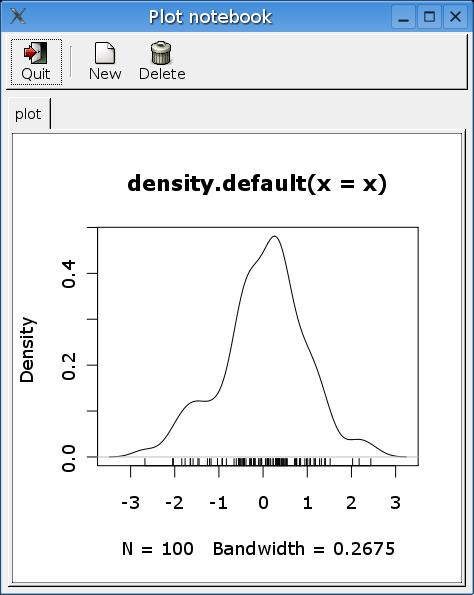
\includegraphics[width=.6\textwidth]{notebook}
  \caption{Notebook widget for holding multiple plot devices provided by \RFunc{ggraphics}}
  \label{fig:notebook}
\end{figure}

That's it (Figure~\ref{fig:notebook}). There is one thing that should
be added. If you switch tabs, the active device does not switch. This
happens though if you click in the plot area. To remedy this, you can
think about the \RFunc{addhandlerchanged} method for the notebook, or
just use \RFunc{ggraphicsnotebook}.

\section{The tree widget}

The \RFunc{gtree} constructor is used to present tree-like data. A
familiar example of such data is the directory structure of your
computer. To describe a tree, \RFunc{gtree} has the idea of a node
which consists of a path back to a root node. This node can have
offspring which will be determined by a function (\RFunc{offspring})
which takes the current path, and a passed in parameter as
arguments. These offspring can either have subsequent offspring or
not. This information must be known at the time of displaying the current
offspring, and is answered by a function (\RFunc{hasOffspring}) which
takes as an argument the offspring. In our file-system  analogy, \RFunc{offspring}
would list the files and directories in a given directory, and
\RFunc{hasOffspring} would be \RCode{TRUE} for a directory in this
listing, and \RCode{FALSE} for a file. For decorations, a function
\RFunc{icon.FUN} can be given to decide what icon to draw for which
listing.

The data presented for the offspring is a data frame, with one column
determining the path. This is typically the first column, but can be
set with \RArg{chosencol}.
\\


To illustrate, we create a file system browser using
\RFunc{gtree}.

First to define the \RFunc{offspring} function we use the
\RFunc{file.info} function. The current working directory is used as
the base node for the tree:

\begin{Schunk}
\begin{Sinput}
> offspring = function(path, user.data = NULL) {
+     if (length(path) > 0) 
+         directory = paste(getwd(), "/", paste(path, sep = "/", 
+             collapse = ""), sep = "", collapse = "")
+     else directory = getwd()
+     tmp = file.info(dir(path = directory))
+     files = data.frame(Name = rownames(tmp), isdir = tmp[, 2], 
+         size = as.integer(tmp[, 1]))
+     return(files)
+ }
\end{Sinput}
\end{Schunk}

The offspring function is determined by the \RCode{isdir} column in
the offspring data frame. 
\begin{Schunk}
\begin{Sinput}
> hasOffspring = function(children, user.data = NULL, ...) {
+     return(children$isdir)
+ }
\end{Sinput}
\end{Schunk}

Finally, an icon function can be given as follows, again using the
\RCode{isdir} column.

\begin{Schunk}
\begin{Sinput}
> icon.FUN = function(children, user.data = NULL, ...) {
+     x = rep("file", length = nrow(children))
+     x[children$isdir] = "directory"
+     return(x)
+ }
\end{Sinput}
\end{Schunk}

The widget is then constructed as follows. See
Figure~\ref{fig:filebrowser} for an example.
\begin{Schunk}
\begin{Sinput}
> gtree(offspring, hasOffspring, icon.FUN = icon.FUN, container = gwindow(getwd()))
\end{Sinput}
\begin{Soutput}
guiWidget of type: gTreeRGtk for toolkit: guiWidgetsToolkitRGtk2 
\end{Soutput}
\end{Schunk}

\begin{figure}[htbp]
  \centering
  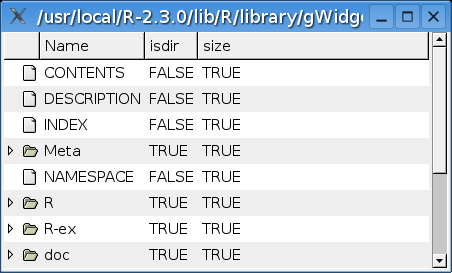
\includegraphics[width=.6\textwidth]{filebrowser}
  \caption{Illustration of a file browser using \RFunc{gtree} constructor.}
  \label{fig:filebrowser}
\end{figure}

The presence of the \RCode{isdir} column may bug some. It was
convenient when defining \RFunc{hasOffspring} and \RFunc{icon.FUN},
but by then had served its purpose. One way to eliminate it, is to use
the default for the \RArg{hasOffspring} argument which is to look for
the second column of the data frame produced by \RFunc{offspring}. If
this is logical, it is used to define \RFunc{hasOffspring} and is then
eliminated from the display. That is, the following would produce the
desired file browser:

\begin{Schunk}
\begin{Sinput}
> gtree(offspring, icon.FUN = icon.FUN, container = gwindow(getwd()))
\end{Sinput}
\begin{Soutput}
guiWidget of type: gTreeRGtk for toolkit: guiWidgetsToolkitRGtk2 
\end{Soutput}
\end{Schunk}

Finally, the  \RArg{handler} argument (or
\RCode{addhandlerdoubleclick}) could have been used to give an action to double
clicking of an item in the tree. 



\section{Popup menus}

A popup menu ``pops'' up a menu after a mouse click, typically a right
mouse click. Implemented here are the functions

\begin{description}
\item[\RFunc{add3rdmousepopupmenu}] for adding a popup on a right click
\item[\RFunc{addpopupmenu}] for adding a popup on any click
\end{description}

The menu is specified using the syntax for \RFunc{gmenu}.
\\


A simple example would be something like:

\begin{Schunk}
\begin{Sinput}
> group = ggroup(container = gwindow("Click on button to change"))
> glabel("Hello ", container = group)
\end{Sinput}
\begin{Soutput}
guiWidget of type: gLabelRGtk for toolkit: guiWidgetsToolkitRGtk2 
\end{Soutput}
\begin{Sinput}
> world = gbutton("world", container = group)
> lst = list()
> lst$world$handler = function(h, ...) svalue(world) <- "world"
> lst$continent$handler = function(h, ...) svalue(world) <- "continent"
> lst$country$handler = function(h, ...) svalue(world) <- "country"
> lst$state$handler = function(h, ...) svalue(world) <- "state"
> addpopupmenu(world, lst)
\end{Sinput}
\end{Schunk}
Clicking on ``world'' with the mouse allows one to change the value in
the label.

\section{Making  widgets from an R function}

A common task envisioned for \RPackage{gWidgetsRGtk} is to create GUIs
that make collecting the arguments to a function easier. Presented
below are two ways to do so without having to do any programming,
provided you are content with the layout and features provided.

One can make an ok GUI for a function without too much work using
\RPackage{gWidgetsRGtk}. We illustrate two ways. First with the
\RFunc{ggenericfunction} constructor and then with a do-it yourself
approach. 


\subsection{Using \RFunc{ggenericwidget}}
\label{sec:using-ggenericwidget}


The \RFunc{ggenericwidget} constructor maps a list into a widget. The
list contains two types of information: meta information about the
widget, such as the name of the function, a help page and information about the widgets. This is specified using a list whose first component is the constructor, and subsequent components are fed to the constructor.

To illustrate, a GUI for a one sample t-test  is given. The
list used by \RFunc{ggenericwidget}  is defined below.

\begin{Schunk}
\begin{Sinput}
> lst = list()
> lst$title = "t.test()"
> lst$help = "t.test"
> lst$variableTypes = "univariate"
> lst$action = list(beginning = "t.test(", ending = ")")
> lst$arguments$hypotheses$mu = list(type = "gedit", text = 0, 
+     coerce.with = as.numeric)
> lst$arguments$hypotheses$alternative = list(type = "gradio", 
+     items = c("'two.sided'", "'less'", "'greater'"))
\end{Sinput}
\end{Schunk}

This list is then given to the constructor.
\begin{Schunk}
\begin{Sinput}
> ggenericwidget(lst, container = gwindow("One sample t test"))
\end{Sinput}
\begin{Soutput}
guiWidget of type: gGenericWidgetRGtk for toolkit: guiWidgetsToolkitRGtk2 
\end{Soutput}
\end{Schunk}

Although this looks intimidating, due to the creation of the list,
there is a function \RFunc{autogenerategeneric} that reduces the work involved.


\subsection{An alternative to \RFunc{ggenericwidget}}
\label{sec:an-altern-ggenericwidget}

This next example shows a different (although ultimately similar) way
to produce a widget for a function. One of the points of this example
is to illustrate the power of having common method names for the
different widgets. Of course, the following can be improved. Two obvious
places are the layout of the automagically generated widget, and and
the handling of the initial variable when a formula is expected.

\begin{Schunk}
\begin{Sinput}
> Comment("A constructor to automagically make a GUI for a function")
> gfunction = function(f, window = gwindow(title = fName), ...) {
+     Comment("Get the function and its name")
+     if (is.character(f)) {
+         fName = f
+         f = get(f)
+     }
+     else if (is.function(f)) {
+         fName = deparse(substitute(f))
+     }
+     Comment("Use formals() to define the widget")
+     lst = formals(f)
+     Comment("Hack to figure out variable type")
+     type = NULL
+     if (names(lst)[1] == "x" && names(lst)[2] == "y") {
+         type = "bivariate"
+     }
+     else if (names(lst)[1] == "x") {
+         type = "univariate"
+     }
+     else if (names(lst)[1] == "formula") {
+         type = "model"
+     }
+     else {
+         type = NULL
+     }
+     Comment("Make widgets for arguments from formals")
+     widgets = sapply(lst, getWidget)
+     Comment("Add update handler to each widget when changed")
+     sapply(widgets, function(obj) {
+         try(addhandlerchanged(obj, function(h, ...) update()), 
+             silent = TRUE)
+     })
+     Comment("Add drop target to each widget")
+     sapply(widgets, function(obj) try(adddroptarget(obj, handler = function(h, 
+         ...) {
+         svalue(h$obj) <- h$dropdata
+         update()
+     }), silent = TRUE))
+     Comment("Put widgets into a layout container")
+     tbl = glayout()
+     for (i in 1:length(widgets)) {
+         tbl[i, 1] = glabel(names(lst)[i])
+         tbl[i, 2] = widgets[[i]]
+     }
+     Comment("Finalize the layout container")
+     visible(tbl) <- TRUE
+     Comment("Main group")
+     gp = ggroup(horizontal = TRUE, container = window)
+     Comment("Arrange widgets with an output area")
+     add(gp, tbl)
+     gseparator(horizontal = FALSE, container = gp)
+     outputArea = gtext()
+     add(gp, outputArea, expand = TRUE)
+     Comment("In case this doesn't get exported")
+     svalue.default = function(obj, ...) obj
+     Comment("Function used to weed out 'NULL' values to widgets")
+     isNULL = function(x) ifelse(class(x) == "character" && length(x) == 
+         1 && x == "NULL", TRUE, FALSE)
+     Comment("Function called when a widget is changed")
+     Comment("2nd and 3rd lines trim out non-entries")
+     update = function(...) {
+         outList = lapply(widgets, svalue)
+         outList = outList[!sapply(outList, is.empty)]
+         outList = outList[!sapply(outList, isNULL)]
+         outList[[1]] = svalue(outList[[1]])
+         if (type == "bivariate") 
+             outList[[2]] = svalue(outList[[2]])
+         out = capture.output(do.call(fName, outList))
+         dispose(outputArea)
+         if (length(out) > 0) 
+             add(outputArea, out)
+     }
+     invisible(NULL)
+ }
\end{Sinput}
\end{Schunk}

The \RFunc{getWidget} function takes a value from \RFunc{formals}
and maps it to an appropriate widget. For arguments of type
\RCode{call} the function recurses.

\begin{Schunk}
\begin{Sinput}
> getWidget = function(x) {
+     switch(class(x), numeric = gedit(x, coerce.with = as.numeric), 
+         character = gdroplist(x, active = 1), logical = gdroplist(c(TRUE, 
+             FALSE), active = 1 + (x == FALSE)), name = gedit(""), 
+         "NULL" = gedit("NULL"), list = gListOfWidgets(x, name = ""), 
+         call = getWidget(eval(x)), gedit())
+ }
\end{Sinput}
\end{Schunk}

This function defines a separate widget to handle the case where an
argument expects a list. It is written in the \RCode{gWidgetsRGtk} style
including an \RFunc{svalue} method below. The \RFunc{tag} method stores
a value in the widget, similar to setting an attribute. In this case,
the list of widgets stored is consulted by the following \RFunc{svalue} method.

\begin{Schunk}
\begin{Sinput}
> gListOfWidgets = function(lst, name = "", container = NULL, ...) {
+     gp = gframe(text = name, container = container, horizontal = FALSE, 
+         ...)
+     obj = list(ref = gp)
+     class(obj) = c("gListOfWidgets", "gComponent", "gWidget")
+     widgetList = lapply(lst, getWidget)
+     tag(obj, "widgetList") <- widgetList
+     tbl = glayout(container = gp)
+     for (i in 1:length(widgetList)) {
+         tbl[i, 1] = glabel(names(widgetList)[i])
+         tbl[i, 2] = widgetList[[i]]
+     }
+     visible(tbl) <- TRUE
+     return(obj)
+ }
\end{Sinput}
\end{Schunk}

The methods below (\RFunc{svalue}, \RFunc{svalue<-} and
\RFunc{addhandlerchanged})  map the same method to each component
of the list using \RFunc{sapply}.

\begin{Schunk}
\begin{Sinput}
> svalue.gListOfWidgets = function(obj, ...) {
+     lst = lapply(tag(obj, "widgetList"), svalue)
+     return(lst)
+ }
> "svalue<-.gListOfWidgets" = function(obj, ..., value) {
+     if (!is.list(value)) 
+         return(obj)
+     widgetList = getdata(obj, "widgetList")
+     sapply(names(value), function(x) svalue(widgetList[[x]]) <- value[[x]])
+     return(obj)
+ }
> addhandlerchanged.gListOfWidgets = function(obj, handler = NULL, 
+     action = NULL, ...) {
+     widgetList = getdata(obj, "widgetList")
+     sapply(widgetList, function(x) try(addhandlerchanged(x, handler, 
+         action), silent = TRUE))
+ }
\end{Sinput}
\end{Schunk}

We can try this out on the default \RFunc{t.test} function. First we
grab a local copy from the namespace, then call our function. The
widget with an initial value for \RCode{x} is shown in
Figure~\ref{fig:gfunction}.


\begin{Schunk}
\begin{Sinput}
> our.t.test = stats:::t.test.default
> gfunction(our.t.test)
\end{Sinput}
\begin{Soutput}
Define length for x of class:[1] "gEditRGtk"
attr(,"package")
[1] "gWidgetsRGtk2"
Define length for x of class:[1] "gEditRGtk"
attr(,"package")
[1] "gWidgetsRGtk2"
Define length for x of class:[1] "gDroplistRGtk"
attr(,"package")
[1] "gWidgetsRGtk2"
Define length for x of class:[1] "gEditRGtk"
attr(,"package")
[1] "gWidgetsRGtk2"
Define length for x of class:[1] "gDroplistRGtk"
attr(,"package")
[1] "gWidgetsRGtk2"
Define length for x of class:[1] "gDroplistRGtk"
attr(,"package")
[1] "gWidgetsRGtk2"
Define length for x of class:[1] "gEditRGtk"
attr(,"package")
[1] "gWidgetsRGtk2"
Define length for x of class:[1] "gEditRGtk"
attr(,"package")
[1] "gWidgetsRGtk2"
\end{Soutput}
\end{Schunk}

\begin{figure}[htbp]
  \centering
  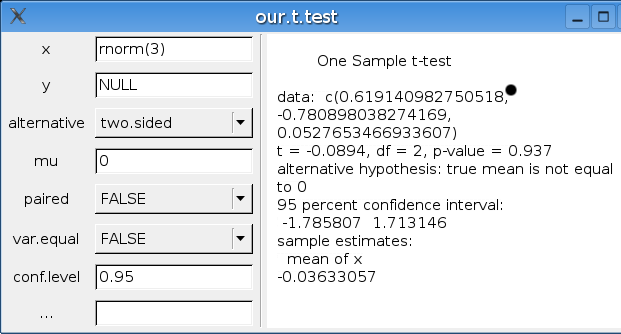
\includegraphics[width=.6\textwidth]{gfunction}
  \caption{Illustration of \RFunc{gfunction}}
  \label{fig:gfunction}
\end{figure}





\end{document}
